\documentclass[10pt]{article}
\usepackage[utf8]{inputenc} 
\usepackage{amssymb}
\usepackage{bm}
\usepackage{latexsym}
\usepackage{amsmath}
\usepackage{url}
\usepackage{cancel}
\usepackage{graphicx}
\newcommand{\indep}{\rotatebox[origin=c]{90}{$\models$}}
\usepackage{hyperref}
\hypersetup{
    bookmarks=true,         
    unicode=true,  
    colorlinks=true,       
    linkcolor=blue,          
    citecolor=blue,       
    filecolor=blue,      
    urlcolor=blue          
}
\DeclareMathOperator*{\argmin}{\arg\!\min}
\DeclareMathOperator*{\argmax}{\arg\!\max}
\newcommand{\ones}{\mathbf 1}
\newcommand{\symm}{{\mbox{\bf S}}}  % symmetric matrices
\usepackage{multirow}
\usepackage{multicol}
\usepackage{calc}

\usepackage{pstricks-add}
% Formatting
\usepackage{geometry}
\geometry{hmargin=1.5cm,vmargin=1.5cm}
\setlength{\parindent}{0pt}
\everymath{\displaystyle}
\renewcommand{\baselinestretch}{1.1}

\usepackage[ruled,vlined]{algorithm2e}

\begin{document}

\noindent
\framebox[\textwidth]{\vbox to 0.8in{
\hbox to\textwidth{~\rlap{\textbf{Probabilistic graphical models, 2015-2016}}
	\hfil\llap{{Master MVA, ENS Cachan~}}}
\medskip
\hbox to \textwidth{\Large\hfill Project progress report \hfill}
\medskip
\hbox to \textwidth{~\rlap{J\'er\^ome DOCKES, \texttt{jdockes@ens-cachan.fr}} \hfill}
\vss
\hbox to \textwidth{~\rlap{Pascal LU, \texttt{pascal.lu@student.ecp.fr}} \hfill}
}}

\medskip

We are mainly based on the research paper \emph{Latent Dirichlet allocation} written by D. Blei, A. Ng, and M. Jordan and published in \emph{Journal of Machine Learning Research}, 3:993-1022, January 2003.

\begin{center}
\textsc{\Large{Presentation of the model}}
\end{center}

We consider a corpus $D$ composed of $|D|$ documents, $k$ topics and a vocabulary list $V$.

Latent Dirichlet allocation (LDA) is a generative probabilistic model of a corpus. The basic idea is that documents are represented as random mixtures over latent topics, where each topic is characterized by a distribution over words. 

LDA is based on the computation of the parameters $(\alpha, \beta)$ where $\alpha$ is the parameter of the Dirichlet distribution which generates the parameter $\theta$ for the multinomial probability distribution over topics in the document and $\beta$ gives the probability that a given topic will generate a certain word: $\beta_{ij}= p(w^j = 1 | z^i = 1)$.

To compute $(\alpha, \beta)$, the idea is to introduce, for each document $d$, $\gamma^{(d)}$ (the variational parameter for the Dirichlet distribution), $\phi^{(d)}$ (the variational parameter for the multinomial distribution, matrix of size number of words in document $d$ $\times$ number of topics) and $w^{(d)}$ contains the number of times each word in the vocabulary appears in the document.

\begin{figure}[ht!]
\begin{center}
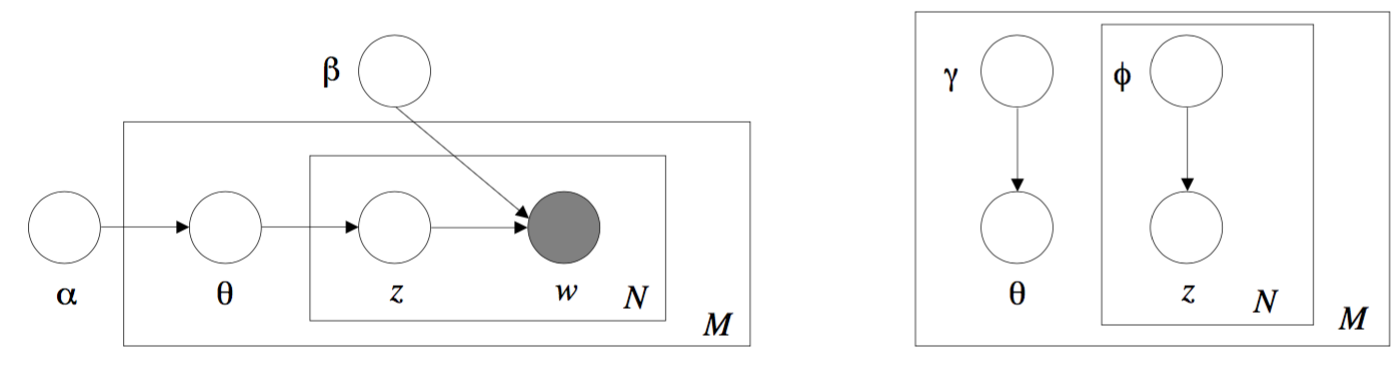
\includegraphics[width=10cm]{fig1.png}
\caption{(Left) Graphical model representation of LDA. (Right) Graphical model representation of the variational distribution used to approximate the posterior in LDA}
\end{center}
\end{figure}

\begin{center}
\textsc{\Large{Main principle of the algorithm}}
\end{center}

The algorithm is based on a variational expectation-maximization algorithm.

\begin{algorithm}
\caption{E-step for a document $d$}
\KwData{\texttt{word$\_$incidences} ($w^{(d)}$), \texttt{dirich$\_$param} ($\alpha$), \texttt{word$\_$prob$\_$given$\_$topic} ($\beta$)}
\KwResult{\texttt{var$\_$dirich} ($\gamma^{(d)}$), \texttt{var$\_$multinom} ($\phi^{(d)}$)}
%\Begin{}
\end{algorithm}

\begin{algorithm}
\caption{M-step}
\KwData{$\{$\texttt{word$\_$incidences} ($w^{(d)}$), \texttt{var$\_$dirich} ($\gamma^{(d)}$), \texttt{var$\_$multinom} ($\phi^{(d)}$), $d \in D\}$}
\KwResult{\texttt{dirich$\_$param} ($\alpha$), \texttt{word$\_$prob$\_$given$\_$topic} ($\beta$)}
\end{algorithm}

\begin{center}
\textsc{\Large{Implementation and problems}}
\end{center}

The preprocessing step (which reads the documents) has been implemented. However, the algorithm described earlier has been implemented but contains some bugs.
\begin{itemize}
\setlength\itemsep{-0.2em}
  \item We need to initialize of $\alpha$ and $\beta$ before starting the EM-algorithm. The initialization step still remains a problem.
  \item The computation of $\beta$ was simplified. It is essentially based on the sum of $(\phi^{(d)})^{\top}w^{(d)}$ for $d \in D$.
  \item The computation of $\alpha$ uses a Newton-Raphson algorithm ``$\alpha \leftarrow \alpha - H(\alpha)^{-1}g(\alpha)$". However, the convergence of $\alpha$ depends on the initialization of $\alpha$.
  \item A basic stopping criterion of E-step and M-step (error made by $\alpha$) has been chosen but a more complex stopping criterion must be implemented.
\end{itemize}

\end{document}